\section{A Web App to Assess DL-Based Code Review via CRAB}
\label{sec:webapp}

To maximize the impact and usability of the CRAB benchmark, we developed a web-based application
designed to facilitate the evaluation of deep learning models on code review tasks. The platform
allows researchers to download task-specific datasets, upload model predictions, track progress, and
retrieve detailed performance results.

\subsection{Functional and Non-functional requirements}
\label{sec:req}

\subsubsection{Dataset Download per Task}

Users must be able to download the dataset corresponding to the specific task they want to benchmark
their model on. The web interface allows the selection between two tasks: \emph{comment generation}
and \emph{code refinement}.

\paragraph{Comment Generation Task}

When benchmarking comment generation models, the user receives a JSON file with a structure
described in Listing~\ref{lst:com-gen-input}.

\begin{listing}[!ht]
	\begin{minted}{json}
    {
      "<id_of_the_instance>": {
        "id": "<id_of_the_instance>",
        "files": {
          "<filename1>": "<content_of_file1_at_beginning_of_pr>",
          "<filename2>": "<content_of_file2_at_beginning_of_pr>",
          // ...
        },
        "diffs": {
          "<filename1>": "<diff_of_file_1_to_get_code_state_before_comment>",
          "<filename2>": "<diff_of_file_2_to_get_code_state_before_comment>",
          // ...
        }
      }
    }
    \end{minted}
	\caption{JSON format of comment generation input}
	\label{lst:com-gen-input}
\end{listing}

This format includes the unique identifier of each benchmark instance, the state of the relevant
files at the start of the pull request, and the diffs needed to understand the changes under review.
This information enables models to generate review comments for the code prior to any feedback. For
information on how to upload predictions, refer to Section~\ref{sec:upload}.

\paragraph{Code Refinement Task}

For code refinement, the user receives a JSON file with additional annotations describing the
reviewer’s comment, as can be seen in Listing~\ref{lst:refinement-input}:

\begin{listing}[!ht]
	\begin{minted}{json}
    {
      "<id_of_the_instance>": {
        "id": "<id_of_the_instance>",
        "files": {
          "<filename1>": "<content_of_file1_at_beginning_of_pr>",
          "<filename2>": "<content_of_file2_at_beginning_of_pr>",
          // ...
        },
        "diffs": {
          "<filename1>": "<diff_of_file_1_to_get_code_state_before_comment>",
          "<filename2>": "<diff_of_file_2_to_get_code_state_before_comment>",
          // ...
        },
        "comments": [
          {
            "file": "<filename1>",
            "body": "<comment_on_file1>",
            "from_": "<starting_line_of_comment_range (if applicable, otherwise null)>",
            "to": "<ending_line_of_comment_range (or comment line if no range)>"
          }
        ]
      }
    }
    \end{minted}
	\caption{JSON format of code refinement input}
	\label{lst:refinement-input}
\end{listing}

Note that the \path{comments} field will always contain exactly one comment. This reflects an
intentional design decision made early in the dataset construction process: we restricted the
dataset to pull requests where it is clear that the code changes following the comment were in
response to that single comment. Handling multiple comments per pull request was deemed too complex
at this stage, as it would require reliably assigning each diff hunk to the appropriate comment—a
task that cannot be automated robustly with current tools. One potential improvement for future
iterations would be to perform this assignment manually during the selection phase. Alternatively,
one could attempt to automate the process by prompting a large language model, either hosted locally
or remotely, to infer whether all comments were addressed by the final set of changes and to perform
a best-effort mapping between comments and diffs. This approach would mirror the possible
enhancement to the pipeline discussed in Section~\ref{sec:stat-expanded}, but comes with its own
risks: LLMs may introduce false positives or negatives, which would undermine the benchmark's
reliability. Maintaining a human element in the selection process is therefore essential to ensure
the benchmark remains accurate, consistent, and trustworthy for empirical evaluation. While the
pipeline and benchmarking logic have been written to support multiple comments in principle, several
features would need further development to fully enable that functionality.

\paragraph{Repository Context (Optional)}

For both tasks, users have the option to download contextual information about the repository at the
beginning of the pull request. By default, the archive they receive contains only the JSON file
described above. If the user opts to include context, the archive will also contain a directory
named \path{context}. Inside this directory, for each instance in the dataset, there will be a
compressed archive named after the instance's \path{id}, containing the full state of the repository
at the time the pull request was opened. This structure allows models to leverage project-wide
information, beyond just the files directly touched by the pull request, enabling more sophisticated
analysis and predictions.


\subsubsection{Uploading Predictions}
\label{sec:upload}

The platform allows users to upload their model predictions for evaluation. To ensure compatibility
with the benchmarking pipeline, each task enforces a strict and clearly defined input format.

\paragraph{Comment Generation Task}

Submissions for the comment generation task must consist of a single JSON object mapping each
instance ID to the corresponding predicted comment. The expected format is described in
Listing~\ref{lst:com-gen-pred-format} and a concrete example is given in
Listing~\ref{lst:com-gen-pred-example}.

\begin{listing}[!ht]
    \begin{minted}{json}
    {
        "<id1>": "<predicted_comment1>",
        "<id2>": "<predicted_comment2>"
    }
    \end{minted}
    \caption{JSON format of predictions for comment generation}
    \label{lst:com-gen-pred-format}
\end{listing}



\begin{listing}[!ht]
    \textbf{Example:}
    \begin{minted}{json}
    {
        "1234": "This method lacks null checks.",
        "5678": "Consider renaming this variable for clarity."
    }
    \end{minted}
    \caption{Example of valid comment generation submission}
    \label{lst:com-gen-pred-example}
\end{listing}

Each comment should be a natural language string intended to emulate the behavior of a human
reviewer given the code in that instance.

Once predictions are submitted, the server evaluates them by computing the BLEU score of each
predicted comment against both the original review comment and its paraphrases. As described in
Section~\ref{sec:paraphrases}, incorporating paraphrases into the benchmark allows us to tolerate
diverse but semantically equivalent outputs. This flexibility acknowledges that different phrasings
can convey the same intent, which is critical for fair model evaluation.

The table displayed to the user after the evaluation will only show the maximum BLEU score achieved
for each prediction. This score is the highest among all BLEU scores computed with the original
comment and its paraphrases. In addition, users can download a detailed report showing the full list
of BLEU scores per instance. In this list, the first entry corresponds to the BLEU score against the
original review comment, while the subsequent entries correspond to the paraphrases. For example, to
retrieve the BLEU score for paraphrase at index~$i$, the user should look at position~$i+1$ in the
score list.

\paragraph{Code Refinement Task}

For code refinement, submissions must follow a slightly more complex structure. The input must be a
JSON object mapping each instance ID to a dictionary of modified files. Each file path (relative to
the repository root) maps to the complete new content of that file. The structure can be seen in
Listing~\ref{lst:refinement-pred-format} and a concrete example of a valid submission in
Listing~\ref{lst:refinement-pred-example}. Only full file contents are accepted, partial diffs will
likely cause compilation to fail. Furthermore, all paths must remain within the repository
boundaries; any attempt to write to paths outside the project root leads to immediate rejection of
the instance submission.

\begin{listing}[!ht]
    \begin{minted}{json}
    {
        "<id1>": {
            "<path_file1>": "<content_file1>"
        },
        "<id2>": {
            "<path_file2>": "<content_file2>",
            "<path_file3>": "<content_file3>"
        }
    }
    \end{minted}
    \caption{JSON format of predictions for code refinement}
    \label{lst:refinement-pred-format}
\end{listing}

\begin{listing}[!ht]
    \textbf{Example:}
    \begin{minted}{json}
    {
        "1234": {
            "src/Main.java": "public class Main { /* updated code */ }"
        },
        "5678": {
            "utils/Helper.java": "public class Helper { /* improved logic */ }",
            "utils/Math.java": "public class Math { /* better maths */ }"
        }
    }
    \end{minted}
    \caption{Example of valid submission for code refinement}
    \label{lst:refinement-pred-example}
\end{listing}

Once a submission is received, the server applies the predicted changes by writing each specified
file content to disk, inside the relevant repository snapshot. A security check ensures that no file
paths escape the repository scope. After the injection phase, the server attempts to compile the
repository. If compilation succeeds, the test suite is executed.

At each stage (i.e. file injection, compilation, and testing) failures are detected and logged. If
any step fails, all subsequent steps are skipped for that instance. This conservative execution
model avoids wasting resources (e.g., there's no reason to test a repository that failed to
compile). The user-facing result table presents only the final success or failure status for each
instance. However, a downloadable detailed report includes exact error messages for each failure.
For example, if compilation fails, the report includes the output of the compilation command to help
users understand what went wrong. This design helps participants debug their model behavior without
requiring access to the backend or raw infrastructure.


\subsubsection{Tracking Evaluation Status}

One feature that might not seem essential at first, but quickly proved necessary in practice, is the
ability to track the progress of an ongoing evaluation process, particularly for the code refinement
task.

Intuitively, the comment generation task does not require progress tracking. Even for large
submissions, the evaluation is nearly instantaneous. Each prediction is compared to the original
comment and its paraphrases using a BLEU score, which is computationally cheap. These comparisons
typically complete within milliseconds per instance, and the task scales well even for hundreds or
thousands of inputs.

In contrast, the code refinement task is considerably more demanding. It involves four sequential
steps for each instance:
\begin{enumerate}
    \item Extracting the build handler (e.g., Maven or Gradle) for the repository.
    \item Injecting the submitted changes into the appropriate files on disk.
    \item Compiling the full project.
    \item Executing the test suite.
\end{enumerate}

While the first two steps are relatively quick, despite involving I/O operations such as unpacking
the repository state into a temporary directory and writing updated files to disk, they are still
manageable and barely noticeable in isolation. However, compilation and testing are major sources of
delay. These phases are highly dependent on the size and complexity of the project: larger
repositories with many modules or dependencies can take a significant amount of time to compile and
test.

This latency introduces a practical issue: the user cannot be expected to wait idly in front of
their browser for the evaluation to complete. The full evaluation of a code refinement benchmark
submission can take a non-trivial amount of time (approximately \todoi{time of running full new
benchmark on code refinement}), which makes the need for a robust tracking mechanism obvious.
Furthermore, long-running tasks are susceptible to common disruptions such as browser refreshes,
network instability, or even the user shutting down their machine.

To address this, we implemented a persistent tracking system. When a user submits a code refinement
benchmark for evaluation, they are issued a unique process identifier. This identifier can be used
to query the current status of the evaluation via the web interface. Users can monitor progress in
real time or retrieve the results after the process has completed. If the user closes their browser
or disconnects, they can return later and provide the process ID to retrieve the results.

Completed evaluations are stored on the server for one week. During this period, users can access
their results at any time. After the retention window expires, the data is automatically deleted.
This setup strikes a balance between system resource usage and user convenience, allowing flexible,
asynchronous interaction with the benchmarking infrastructure.

\subsection{Design}

\subsubsection{Frontend}
\label{sec:frontend}

Rather than adopting a complex and bloated frontend framework, we intentionally opted for a simple
and robust solution: a plain HTML page. This choice aligns with the philosophy outlined
in~\cite{justusehtml}, a resource we encountered after the fact but which succinctly captures the
rationale behind our decision. Given the limited user interaction and static nature of the
interface, a minimal HTML design not only avoids unnecessary overhead but also ensures maximum
reliability and maintainability.

\begin{figure}[H]
    \centering
    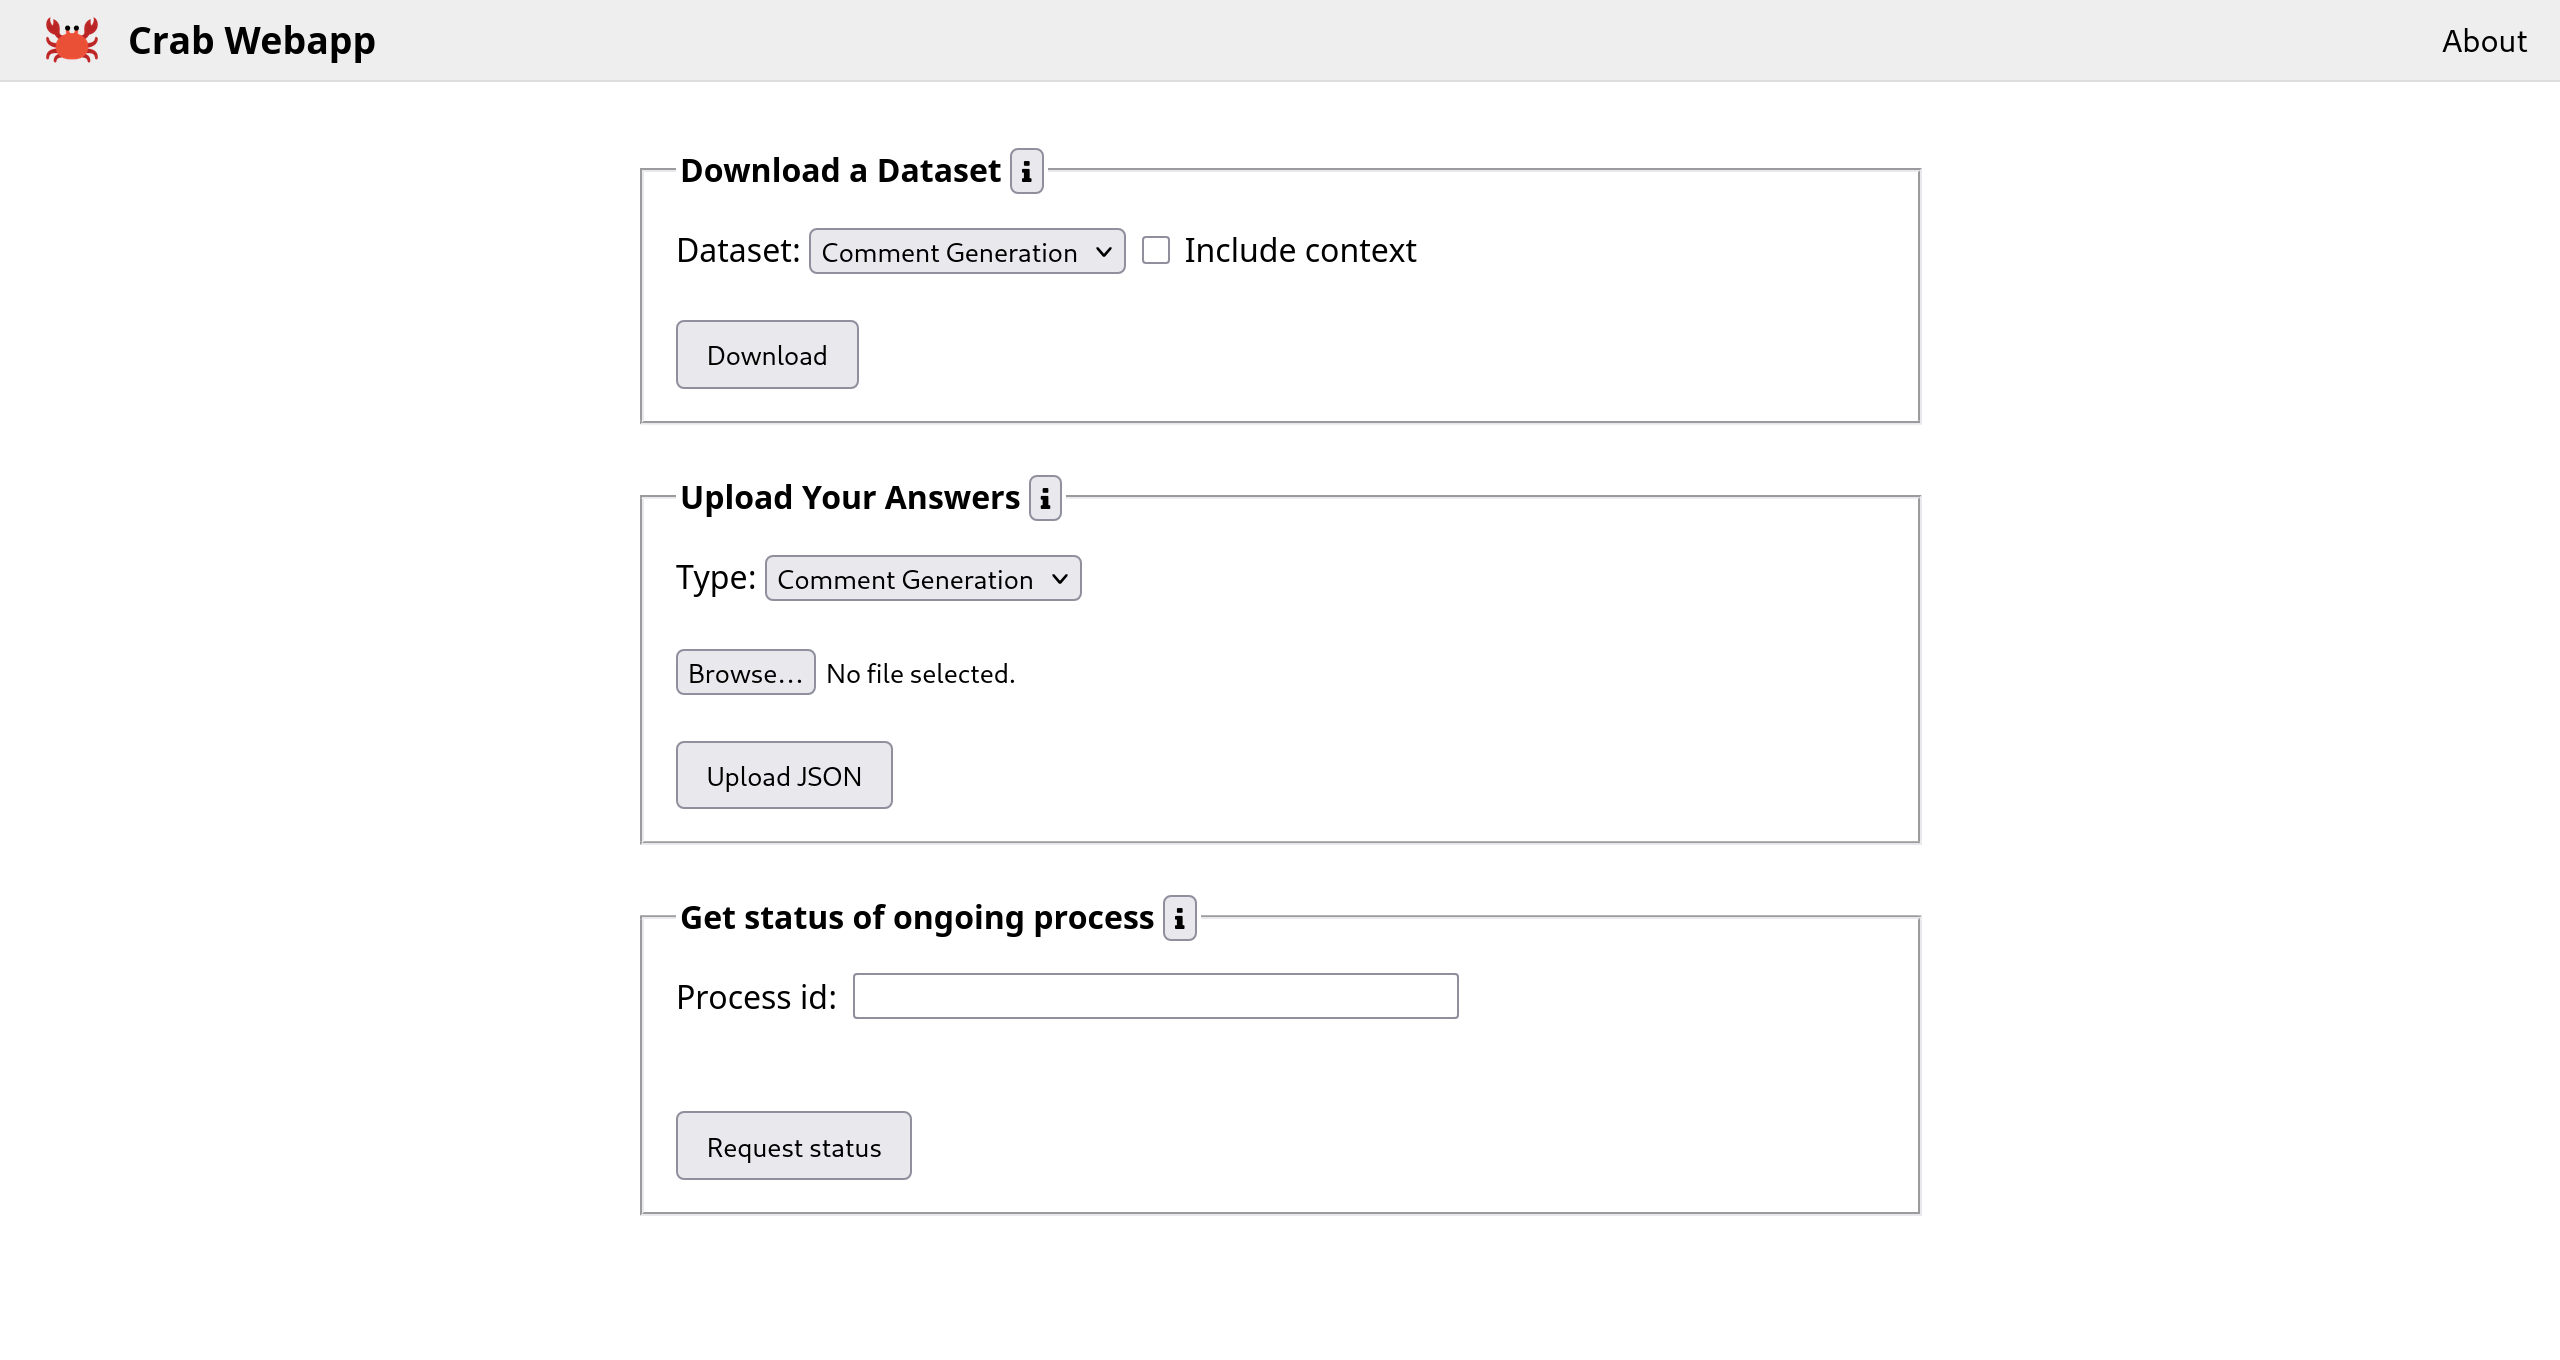
\includegraphics[width=\textwidth,cfbox=black .1pt 0pt]{entire-webiste.png}
    \caption{Main web interface with all three user-facing sections visible}
    \label{fig:full-page}
\end{figure}

The interface is divided into three main sections, each corresponding to one step in the user
workflow: downloading input data, uploading model predictions, and retrieving evaluation results, as
shown in Figure~\ref{fig:full-page}.

\paragraph{Downloading Input Data}

The first section allows users to download the input data corresponding to the benchmark tasks. A
dropdown menu enables the selection between \textit{Comment Generation} and \textit{Code
Refinement}. Once selected, the user can download a ZIP archive containing a JSON file in the
structure described in Section~\ref{sec:req}, along with the optional repository context if
selected. The context includes the full state of the repository at the beginning of the pull
request, which can be useful for models that benefit from project-wide information.

\paragraph{Uploading Predictions}

The second section is used to upload predictions generated by the user's model. As detailed in
Section~\ref{sec:req}, submissions must follow a strict schema depending on the selected task. The
frontend ensures that the uploaded file is correctly received and passed to the backend. If the file
is well-formed, the backend responds with a unique process identifier.

\begin{figure}[H]
    \centering
    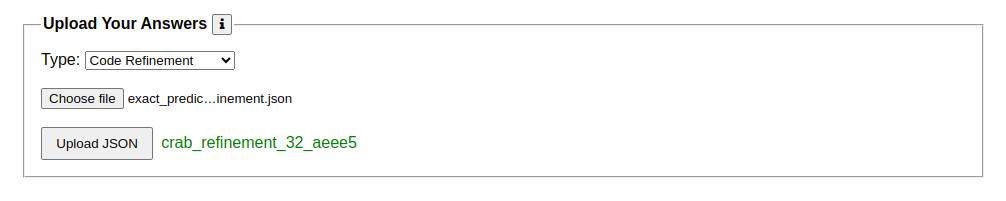
\includegraphics[width=.9\textwidth]{upload-cropped.png}
    \caption{Submission section showing the returned process ID after a successful upload}
    \label{fig:upload-id}
\end{figure}

This ID is displayed directly beside the upload button, as shown in Figure~\ref{fig:upload-id}, and
is crucial for retrieving progress updates and final results. If the user loses the ID, they lose
access to the evaluation process and its results.

\paragraph{Tracking Progress and Viewing Results}

The third section is dedicated to progress tracking and results retrieval. An input field allows
users to enter the process ID. If the user has just submitted a file, this field is pre-populated
with the returned ID. Upon submission, a live progress bar appears, indicating the current status of
the evaluation.

\begin{figure}[H]
    \centering
    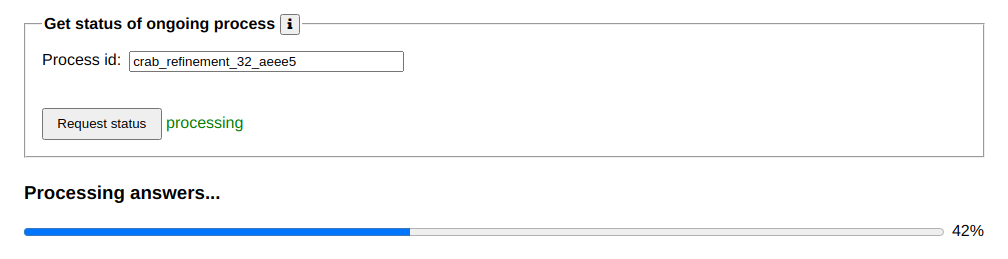
\includegraphics[width=0.9\textwidth]{progress-bar-cropped.png}

    \todo{fix this image}
    \caption{Progress bar showing real-time status of the evaluation process}
    \label{fig:progress-bar}
\end{figure}


As illustrated in Figure~\ref{fig:progress-bar}, this feature is particularly important for the code
refinement task, where evaluation involves compiling and testing the full repository and can take
several minutes per submission. Once the process concludes, the progress bar is replaced by a
results table.

\paragraph{Comment Generation Results}

For the comment generation task, the results table includes:
\begin{itemize}
    \item The instance ID.
    \item The submitted comment.
    \item A boolean flag indicating whether the predicted comment targeted the correct file.
    \item The distance (in lines) between the predicted comment range and the original.
    \item The maximum BLEU score achieved across the original and paraphrased comments.
\end{itemize}

\begin{figure}[H]
    \centering
    % \includegraphics[width=.9\textwidth]{comment-table-cropped.png}
    \todo{take screenshot of comment gen table (with download button)}
    \caption{Result summary table for comment generation predictions}
    \label{fig:comment-table}
\end{figure}

Figure~\ref{fig:comment-table} shows the result summary. In the top-right corner of the table, a
\textit{Download Results} button allows users to retrieve the detailed evaluation. This is a JSON
file where each instance ID maps to an object containing the prediction, file correctness flag,
range distance, maximum BLEU score, and the full list of BLEU scores. As described in
Section~\ref{sec:req}, the first BLEU score corresponds to the original review comment, and the rest
to its paraphrases.

\paragraph{Code Refinement Results}

The results table for the code refinement task is more concise. It includes:
\begin{itemize}
    \item The instance ID.
    \item A boolean indicating whether compilation succeeded.
    \item A boolean indicating whether all tests passed.
\end{itemize}

\begin{figure}[H]
    \centering
    % 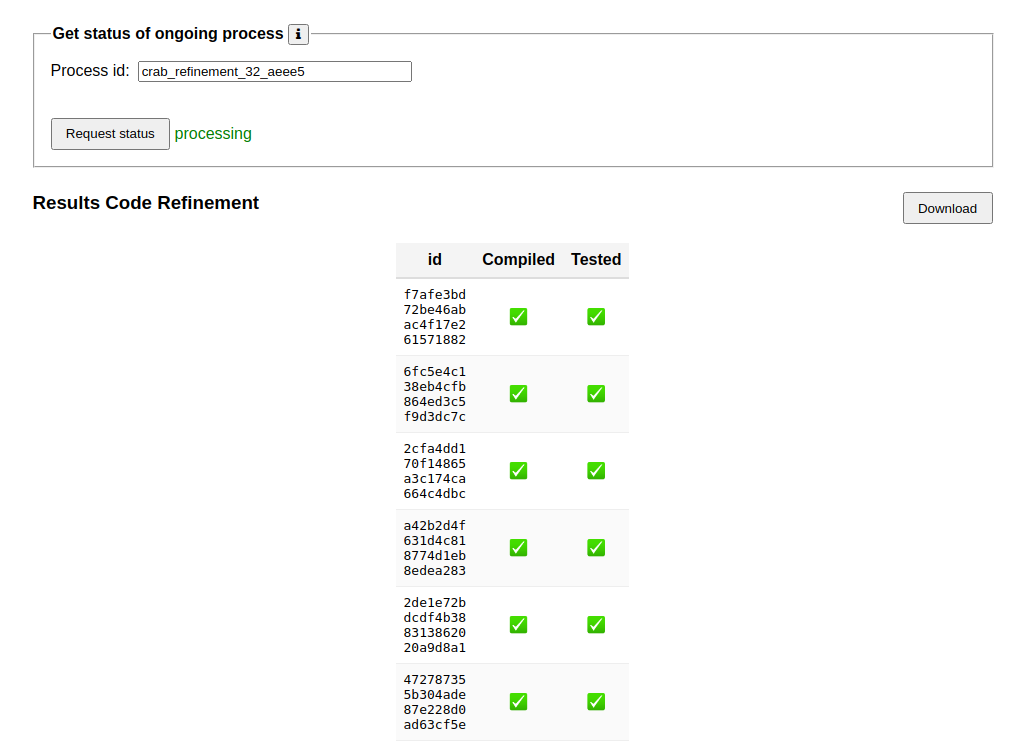
\includegraphics[width=.9\textwidth]{refinement-table-cropped.png}
    \todo{take screenshot of refinement table (with download button)}
    \caption{Result summary table for code refinement predictions}
    \label{fig:refinement-table}
\end{figure}

Figure~\ref{fig:refinement-table} shows the results view for this task. The downloadable detailed
results provide the same boolean indicators along with the failure messages, if any. If an instance
failed to compile, the compilation error output is included. If the tests failed, the test failure
logs are provided. This helps users quickly understand what went wrong and improve their model
accordingly.

Both results tables are fully sortable by any column. This feature enables users to quickly identify
outliers, inspect their worst- and best-performing instances, and iterate on their model behavior
efficiently.


\subsection{Usage Scenarios}

{\color{gray} Show via screenshots how the webapp works with a concrete example.}
\label{sec:refinement} % NOTE: move this thing where it needs to be in the future
\label{sec:paraphrases-check} % NOTE: move this thing where it needs to be in the future
